\documentclass{standalone}
\usepackage{tikz}
\usepackage{ctex,siunitx}
\setCJKmainfont{Noto Serif CJK SC}
\usepackage{tkz-euclide}
\usepackage{amsmath}
\usetikzlibrary{patterns, calc,3d}
\usetikzlibrary {decorations.pathmorphing,decorations.pathreplacing,decorations.shapes}
\begin{document}
\small
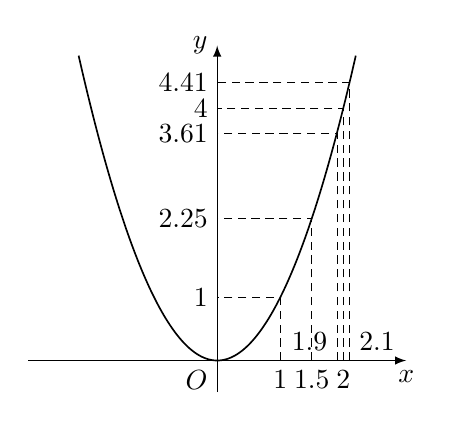
\begin{tikzpicture}[>=latex,scale=0.8]
  \draw[->](-3,0)--(3,0)node[below]{$x$};
  \draw[->](0,-0.5)--(0,5)node[left]{$y$};
  \node at (0,0)[below left]{$O$};
  \draw[semithick,samples=200,domain=-2.2:2.2]plot(\x,\x*\x);
  \foreach \x/\y in {1/1,1.5/2.25,1.9/3.61,2/4,2.1/4.41}
  {
    \draw[very thin,densely dashed](\x,0)--(\x,\y)--(0,\y)node[left]{$\y$};
  }
  \node at (1,0)[below]{1};
  \node at (1.5,0)[below]{1.5};
  \node at (2,0)[below]{2};
  \node at (2.1,0)[above right]{2.1};
  \node at (1.9,0)[above left]{1.9};
\end{tikzpicture}
\end{document}